\section{Lezione del Wed 22 May 2019 03:45:35 PM CEST}
\subsection{Immunit\'a ai disturbi in sistemi analogici}
Principale differenza tra elettronica analogica e digitale \'e  che \'e in grado di distinguere il segnale dal rumore.

\begin{figure}[ht]
    \centering
    \begin{circuitikz}
        \draw(-1, 3) node[nmos] (N1){};
        \draw(1, 3) node[nmos, xscale=-1] (N2){};
        \draw(N1.G) to[short, -o] ++ (-0.2, 0) node[above]{$V_1$};

        \draw (0, 0) node[eground] (G){}
            to[isource] ++ (0, 2) node(bisection){} -- ++ (-1, 0) -- (N1.S);
        \draw (N1.D) to[short, -o] ++ (0.5, 0)
            node[above]{$V_U$};

        \draw(1.2, 1) node[anchor=east]{$\big\uparrow I_0$};
        \draw(N1.D) to[R, -o] ++(0, 2)
            -- ++ (0, 1)
            -- ++ (1, 0)
            node(UB){}
            -- ++ (1, 0)
            -- ++ (0, -1)
            to[R, o-] (N2.D);

        \draw(bisection.center) -- ++ (1,0) -- (N2.S);
        \draw(N2.G) to[short, -o] ++ (0.2, 0) node[above]{$V_2$};

        \draw(UB.center) to[short, ->] ++ (0, 1) node[vdd]{$V_{DD}$};
    \end{circuitikz}
    \caption{Amplificatore Differenziale\label{circuito_1}}
\end{figure}


Osservazioni su Figura~\ref{circuito_1}:
\begin{itemize}
    \item Per Kirkoff $ I_1 + I_2 = I_0$

    \item Siccome la somma delle correnti \'e non nulla, i due transistori ($M_1$  e $M_2$), non possono essere spenti allo stesso tempo

        $I_{D\text{sat}} = \frac{\beta}{2}{(V_{GS}-V_T)}^2$

    \item La caratteristica del generatore di corrente sul piano Tensione-Corrente \'e che \'e costante $\Rightarrow$ la tensione $V_X$ \'e incognita

    \item
        Per Kirkoff:
        $V_1 - V_{GS1} + V_{GS2} - V_{2} = 0 \Rightarrow$
        $V_1 - V_2 = V_{GS1} - V_{GS2}$
\end{itemize}

Supponenedo che per ipotesi: $M_1$ se acceso \'e saturo e $M_2$ Se acceso \'e saturo, e, supponendo che $V_1 = V_2$, allora:

$V_1 - V_2 = 0 \Rightarrow V_{GS2} - V_{GS2} = 0 \Rightarrow V_{GS1} = V_{GS2} $

Siccome la corrente dipende solo da $V_{GS}$, se le tensini sono uguali, le correnti sono uguali $\xrightarrow{SAT} I_1 = I_2$

Siccome $I_1 + I_2 = 0 \Rightarrow I_1 = \frac{I_0}{2} , I_2 = \frac{I_0}{2}$

\[
    V_{U1} = V_{DD} - RI_1 = V_{DD} - R\frac{I_0 }{2}
\]

\[
    V_{U2} = V_{DD} - RI_2 = V_{DD} - R\frac{I_0 }{2}
\]
Il valore di uscita non dipende dall'ingresso, se $V_1$ e $V_2$ sono uguali tra di loro, l'uscita non dipende da loro (Se lavoriamo in regione di saturazione)

Questo tipo di circuito non vede il rumore, siccome entra uguale in entrambi gli ingressi

\vspace{20px}
Supponendo ora che $V_1$ e $V_2$ siano \textbf{diversi}, (es $V_1 > V_2$):

\[
    V_1 - V_2 > 0 \Rightarrow V_{GS1} - V_{GS2} > 0 \Rightarrow V_{GS1} > V_{GS2}
\]
\[
    V_{GS1} > V_{GS2} \Rightarrow I_1 > I_2
\]

Dato che la somma delle correnti \'e limitata ($I_1 + I_2 = I_0$), la corrente $I_1$ continua a crescere, mentre $I_2$ diminuisce, Fino a quando la corrente $I_0$ gira unicamente su un ramo. La corrente non pi\'o diventare negativa perch\'e andrebbe contro le condizioni del transistore.

\begin{figure}[ht]
    \centering
    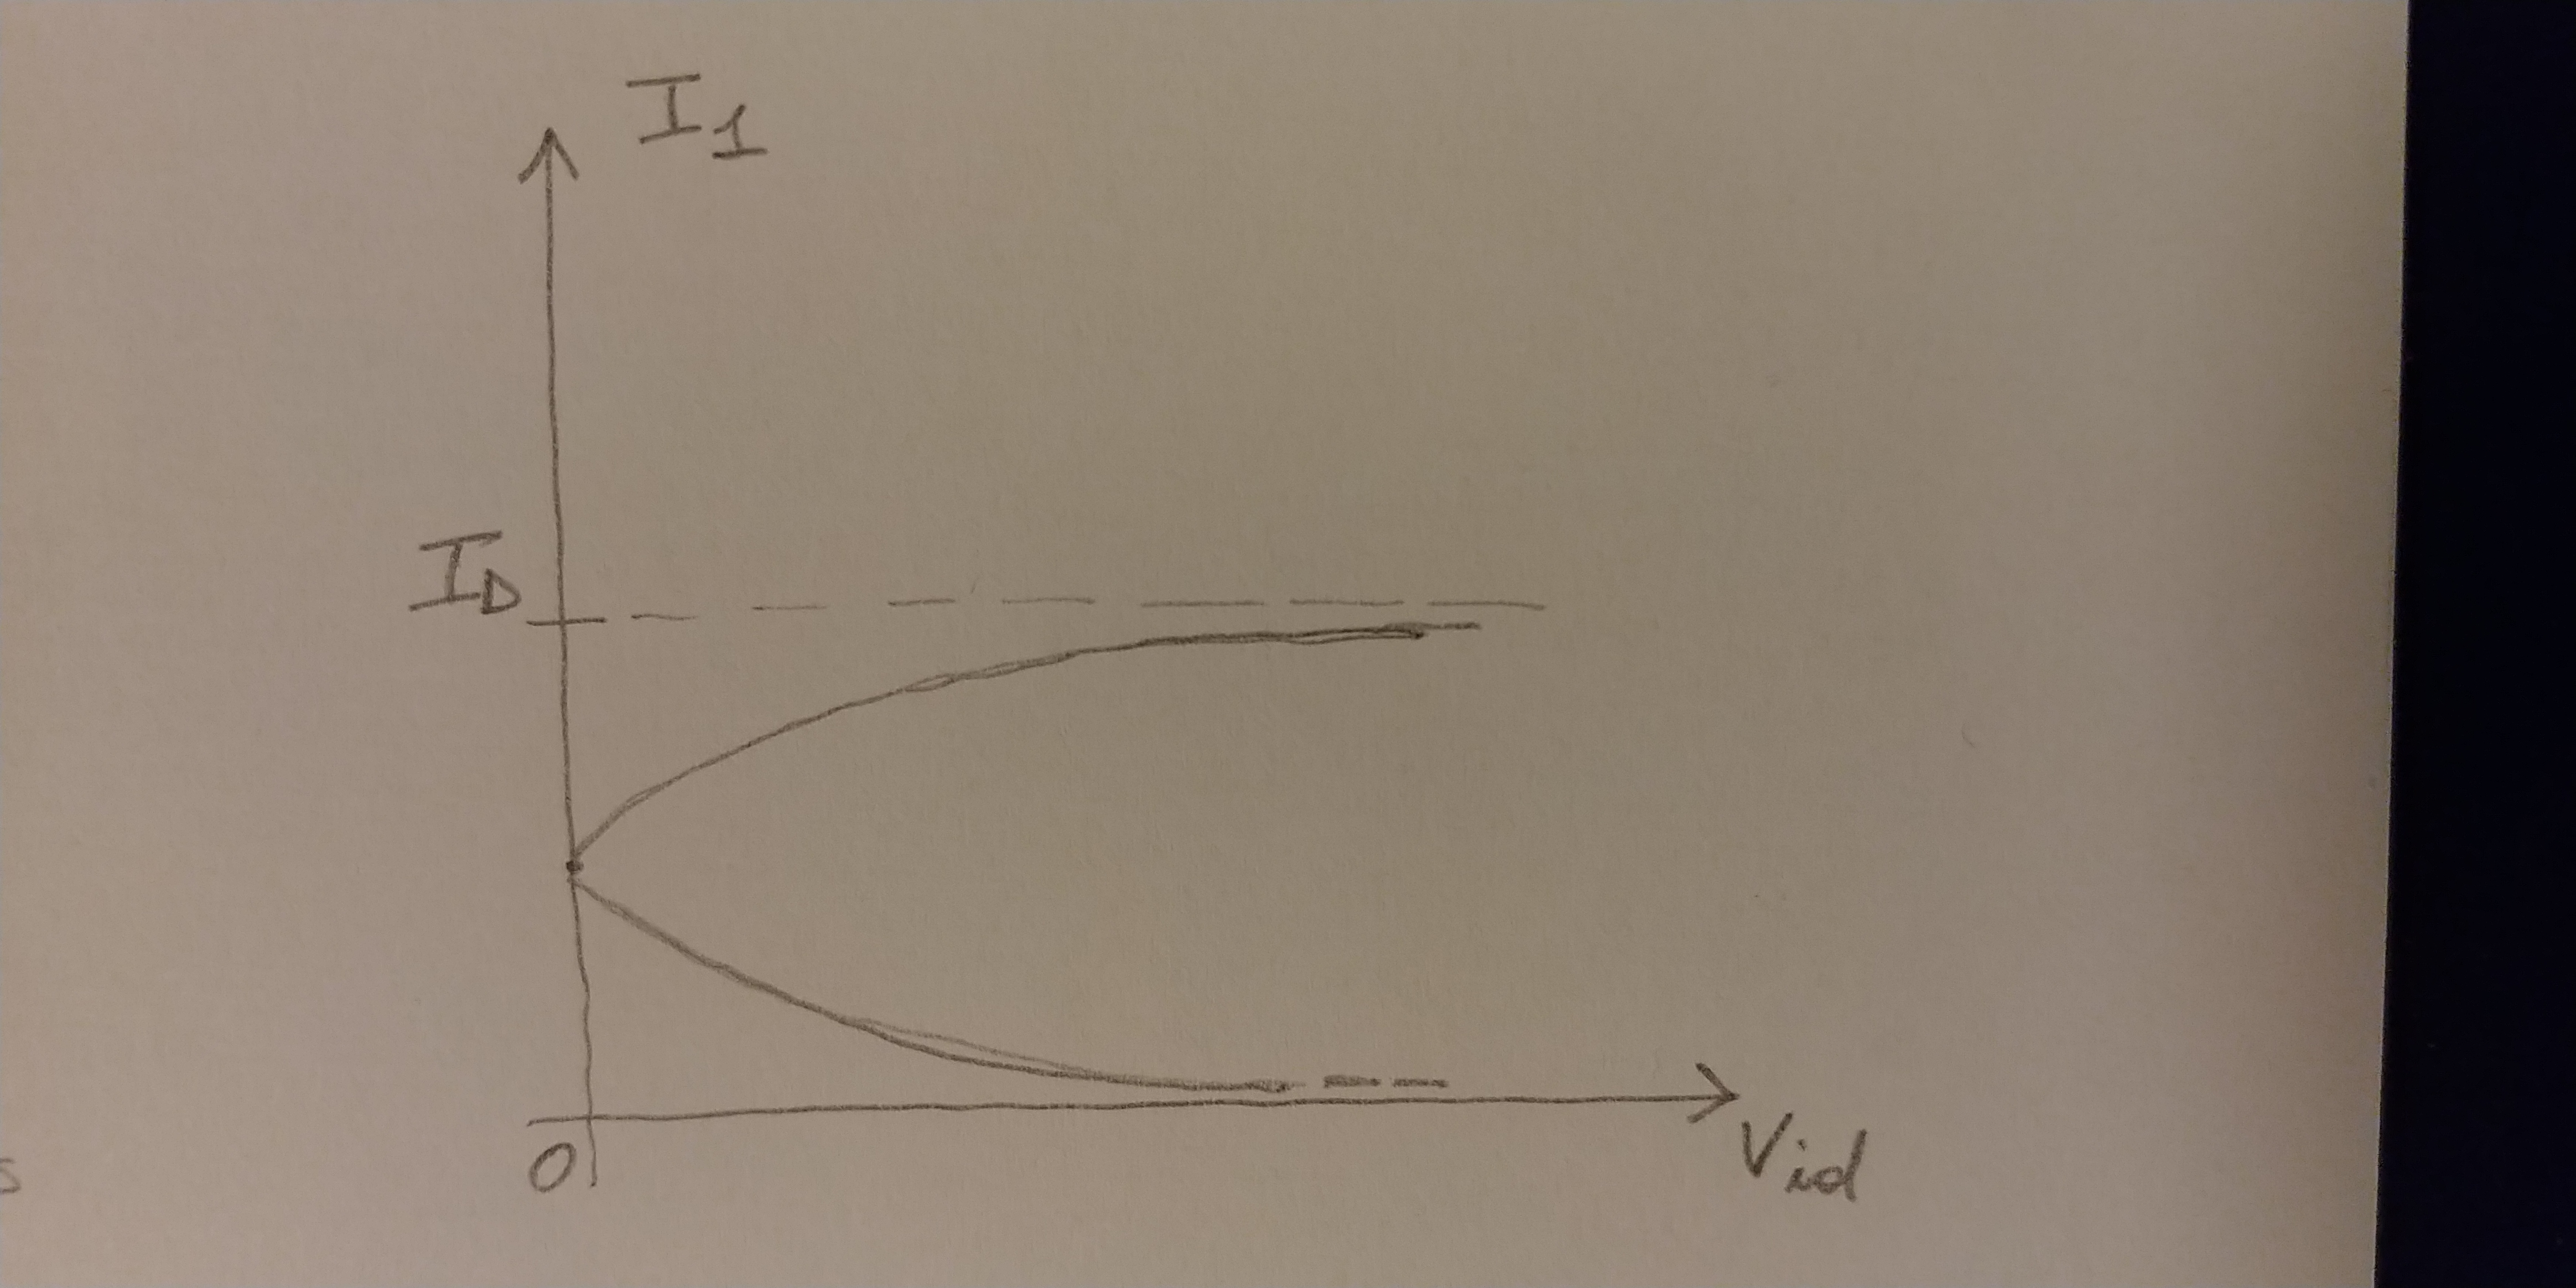
\includegraphics[width=4in]{img/elettronica/grafico2.jpg}
    \caption{Grafico $I_0$, $V_{id}$\label{grafico_analog}}
\end{figure}

Chiamata $V_{iD}$ la tensione differenziale, posso tracciare l'andamento di $I_1$ (Figura~\ref{grafico_analog}), il quale satura al valore $I_0$

\begin{minipage}[t]{0.45\textwidth}
\[
    \begin{cases}
    V_{u1} = V_{DD} - RI_1\\
    V_{u2} = V_{DD} - RI_2
    \end{cases}
\]
\end{minipage}
\begin{minipage}[c]{0.5\textwidth}
    % Grafico
    \begin{center}
        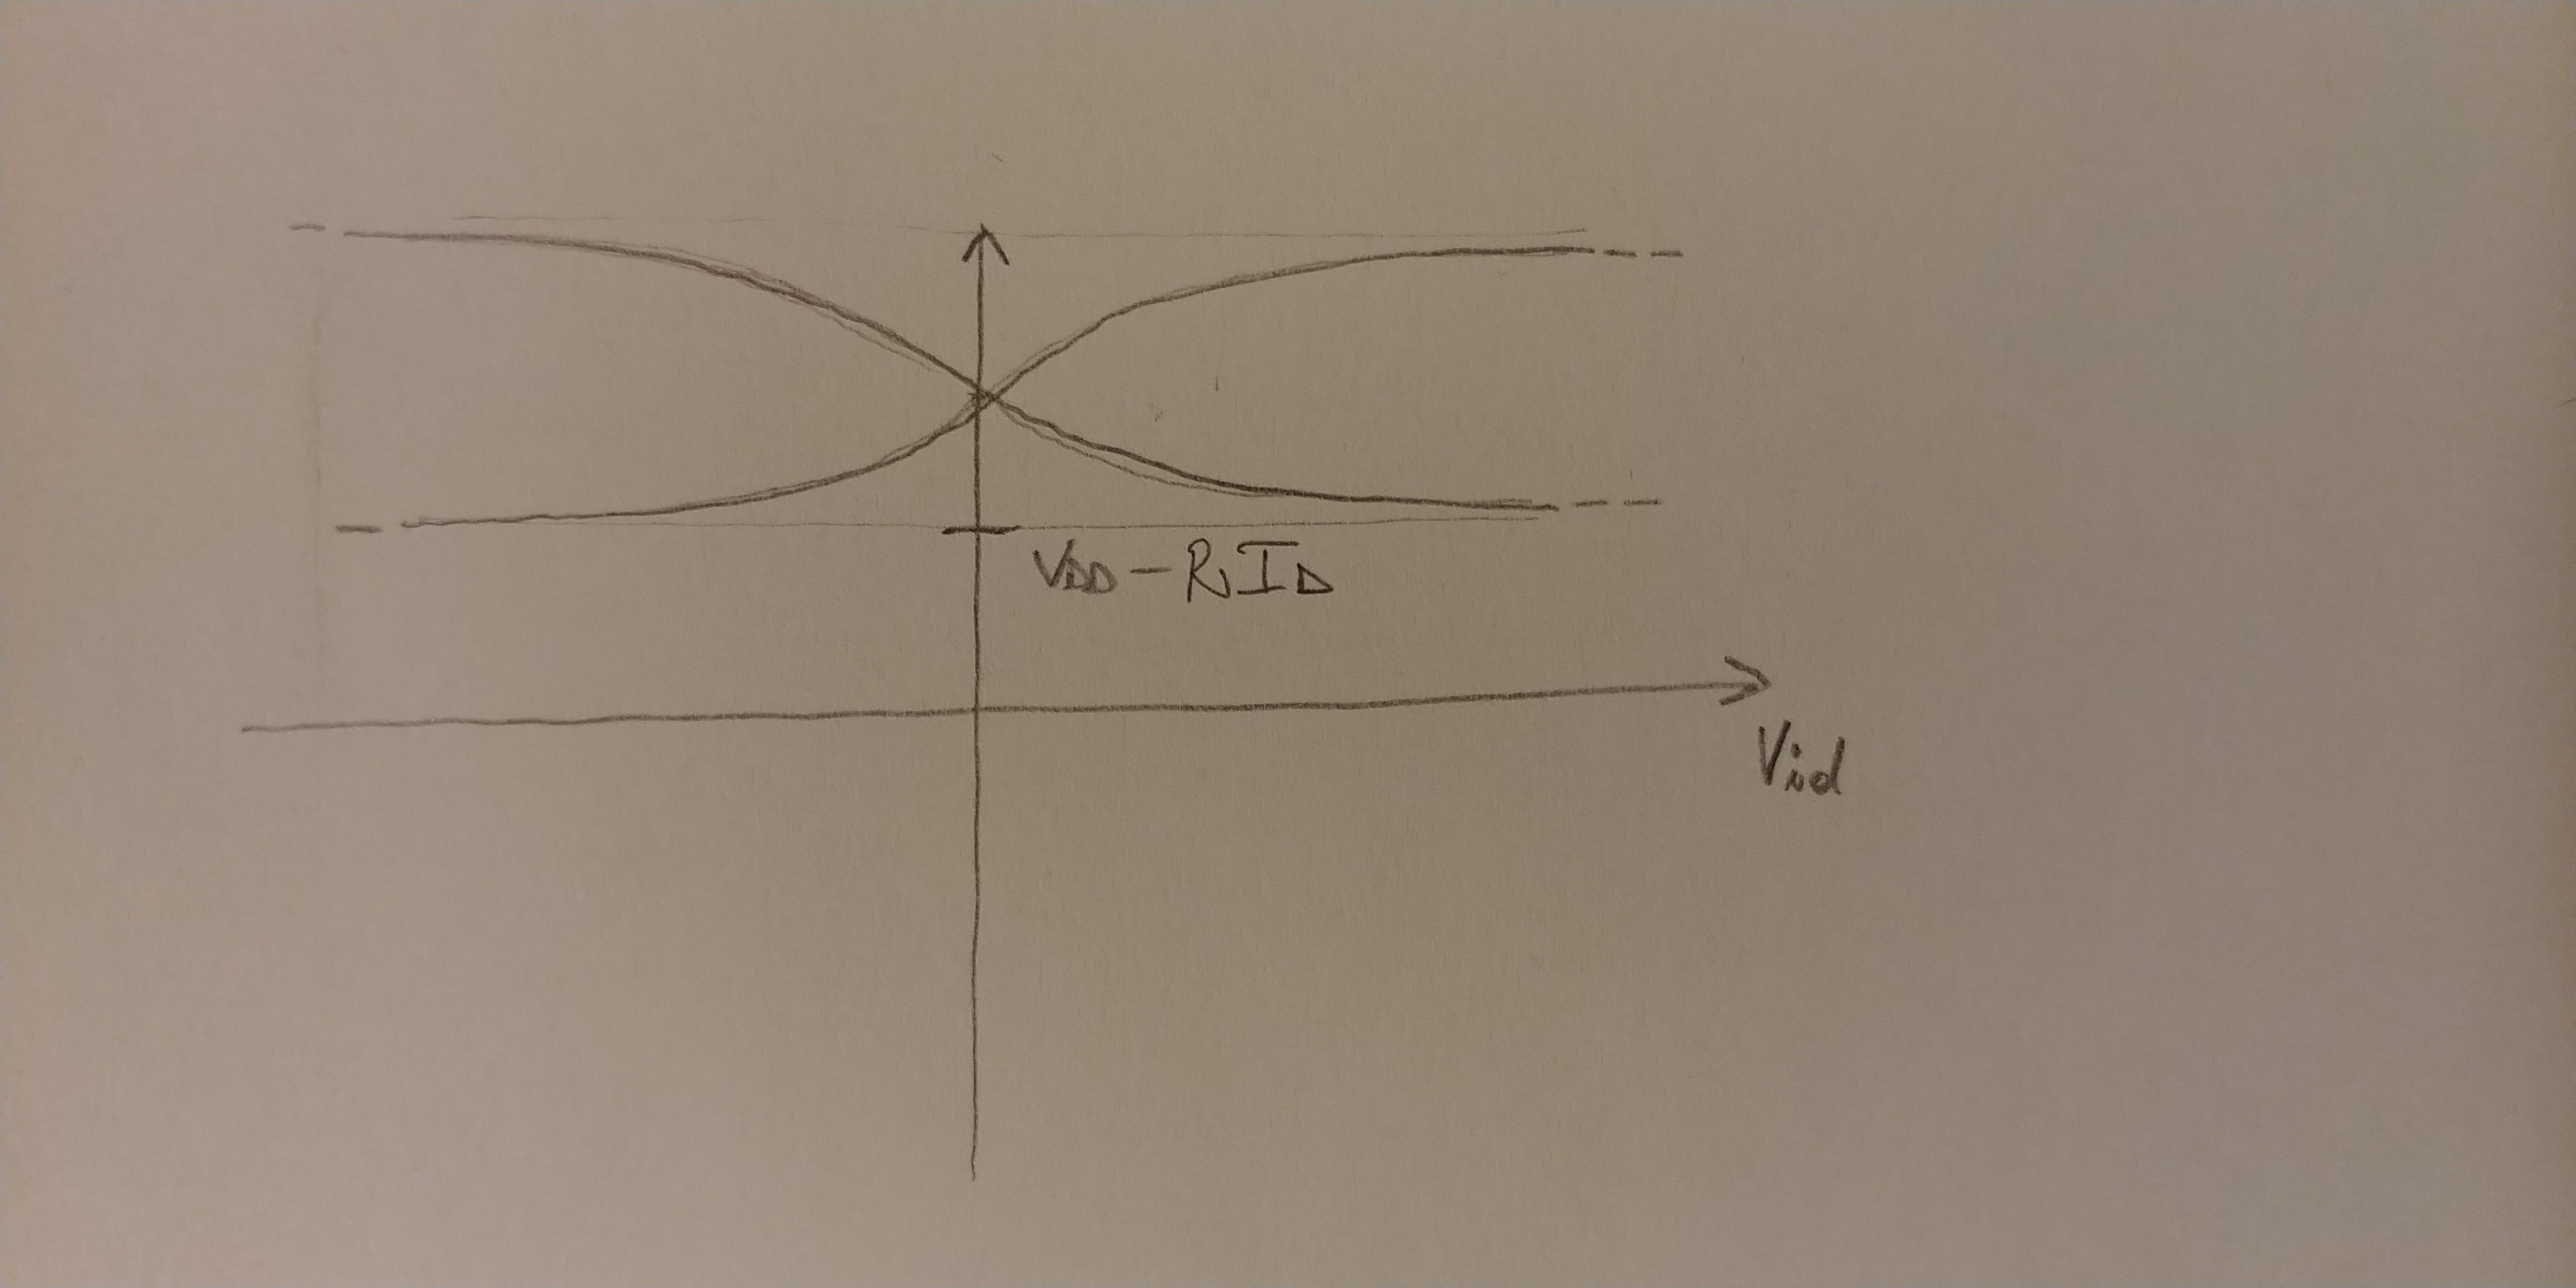
\includegraphics[width=2.8in]{img/elettronica/grafico3.jpg}
    \end{center}
\end{minipage}

Comportamento radicalmente diverso se i segnali variano simultaneamente o non; Quelle non simultanee vengono amplificate

Segnale d'ingresso di modo differenziale
\[
    \begin{cases}
        V_{id} = V_1 - V_2\\
        V_{ic} = \frac{V_1 + V_2}{2}
    \end{cases} \Rightarrow
    \begin{cases}
        V_1 = V_{ic} + \frac{V_{id}}{2} \\
        V_2 = V_{ic} + \frac{V_{id}}{2} - V_{id} = V_{ic} - \frac{V_{id}}{2}
    \end{cases}
\]

Qualunque coppia di segnali \'e suddivisiile in un segnale di modo comune ed un segnale differenziale, questo circuito cancella il segnale di modo comune, mentre il segnale di modo differenziato viene amplificato.

\'E utile per distinguere quale segnale contribuisce all'uscita

\begin{figure}[ht]
\begin{circuitikz}
    \draw(0, 0) node[nmos](Q){};
    \draw(0, -1) node[eground](G){};
    \draw(Q.G) to[short, -o] ++(-0.5, 0) node[above]{$V_i$};

    \draw(Q.D) to[R, -o] ++(0, 2)
        (Q.S) to[-] (G.center);
    \draw(Q.D) to[short, -o] ++(1,0)
        node[above]{$V_u$};
\end{circuitikz}
\end{figure}

Se mettessi in ingresso due volte lo stesso segnale all'amplificatore differenziale (Figura~\ref{circuito_1}):
\[
    V_{ic} = \frac{V_{i0} + \cancel{V_m \sin wt} + V_{i0} - \cancel{V_m \sin wt} - V_{i0}}{2} = V_{i0}
\]

\[
    V_m = \cancel{V_{i0}} + V_m \sin wt - \cancel{V_{i0}} + V_m \sin wt = 2 V_m \sin wt
\]

\subsection{Generatore di corrente}

\begin{figure}[ht]
    \centering
    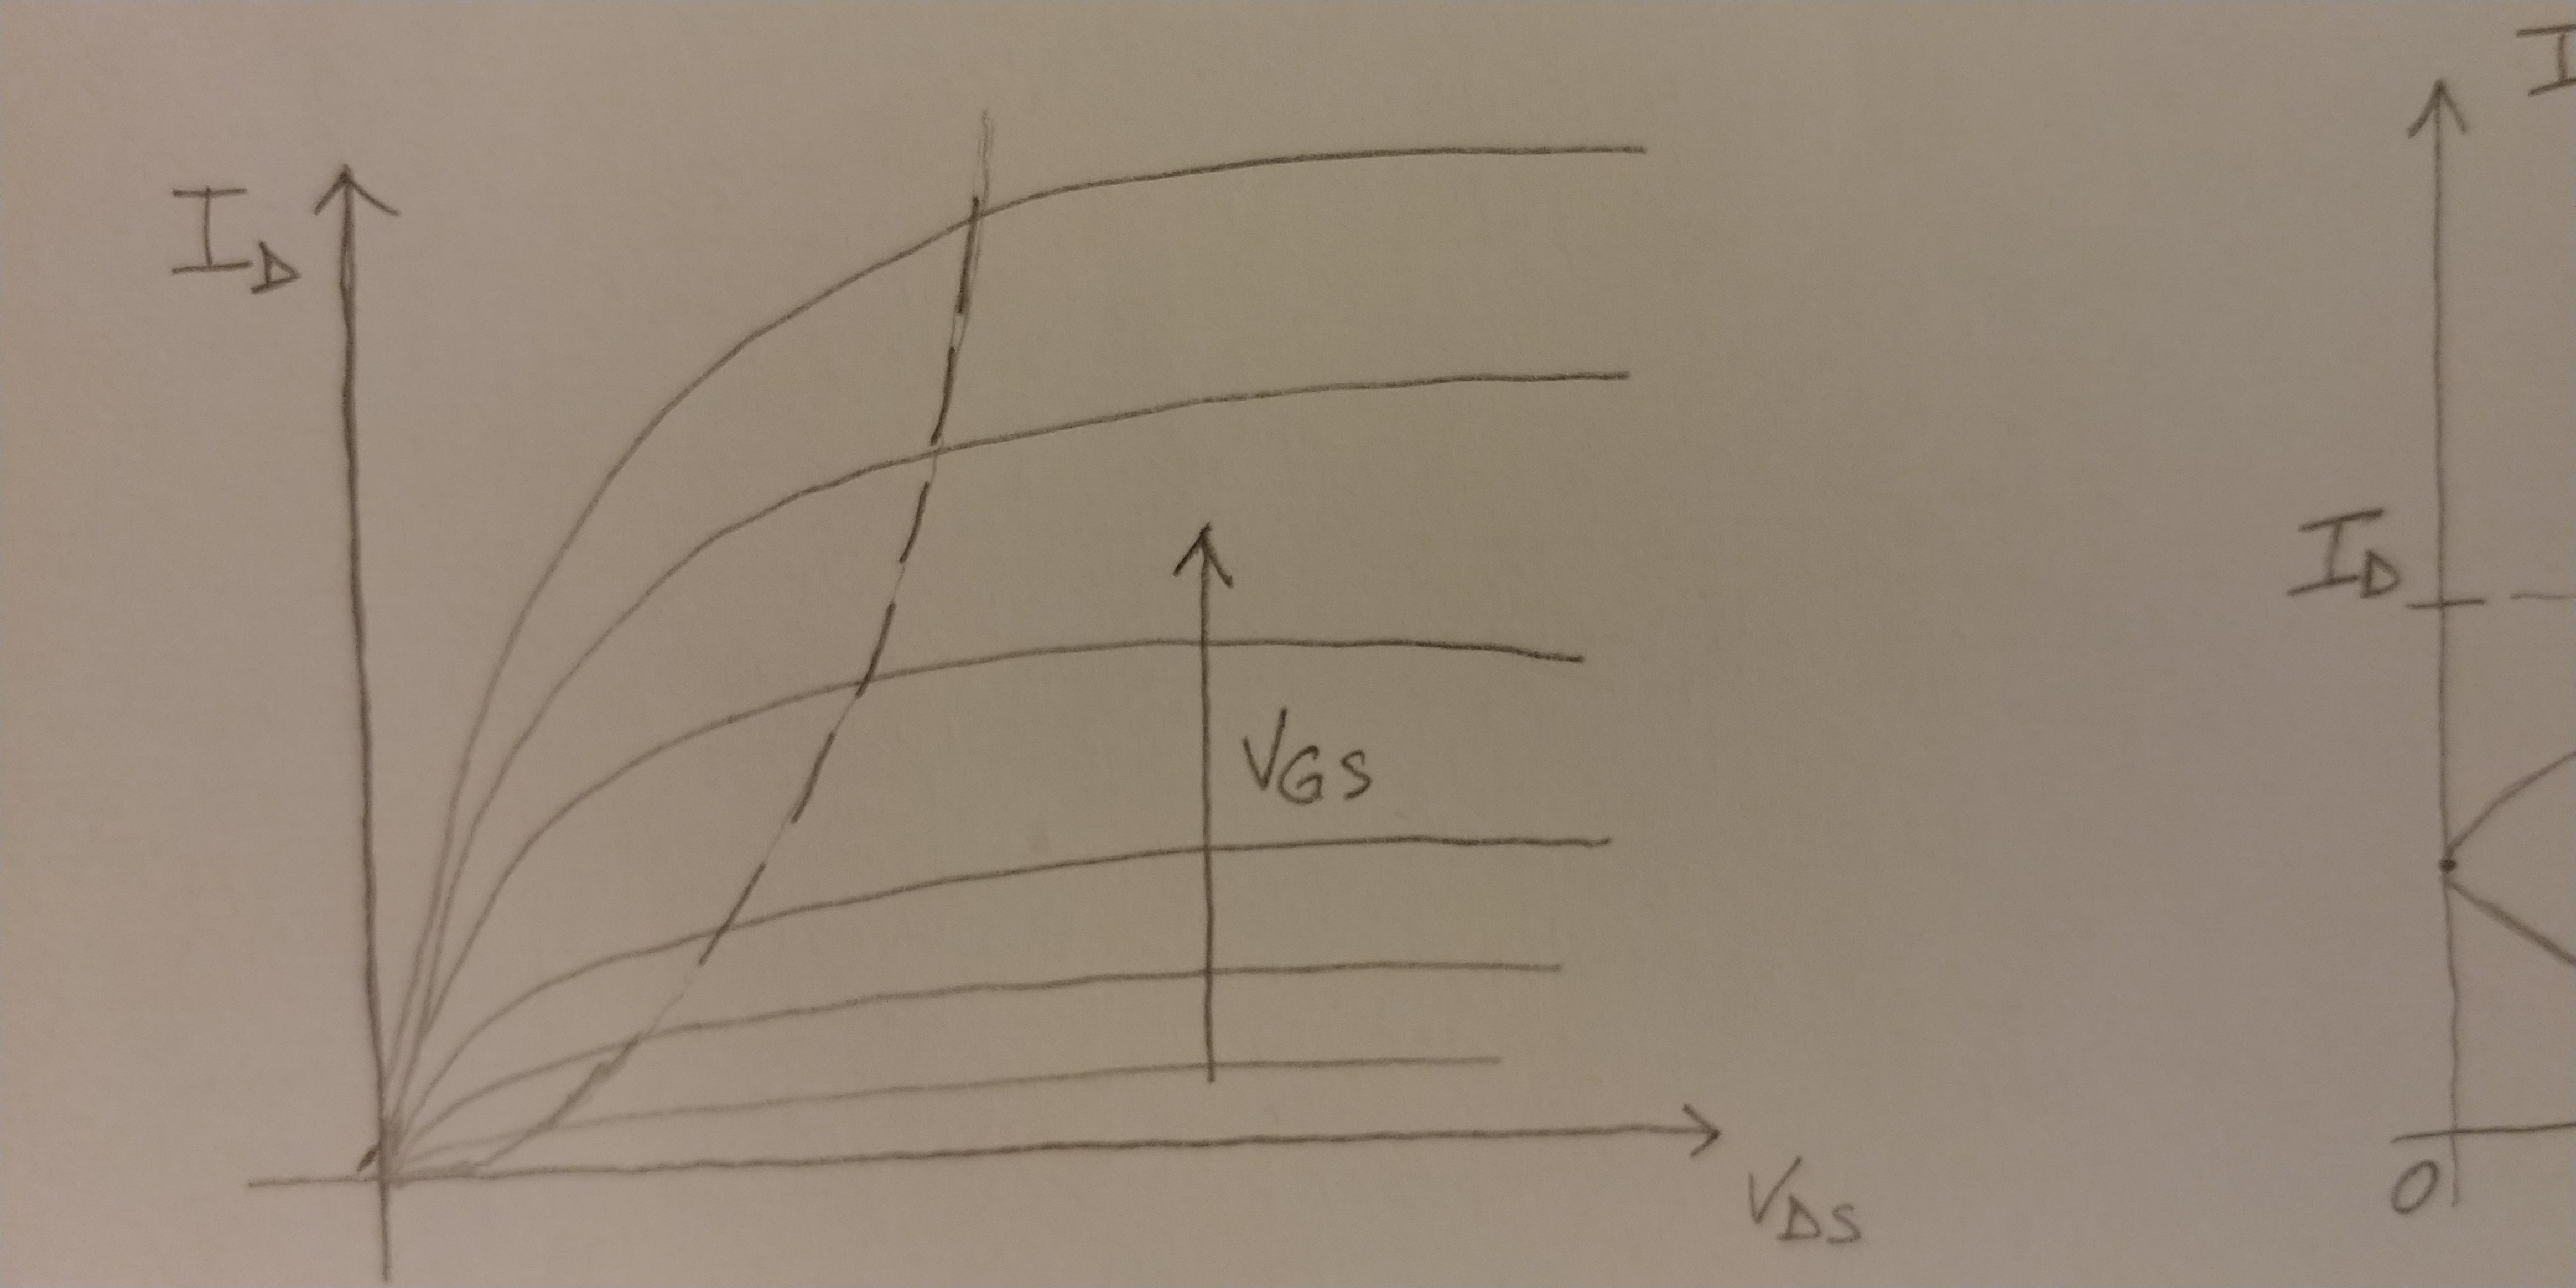
\includegraphics[width=4in]{img/elettronica/grafico1.jpg}
    \caption{Grafico con linee orizzontali}
\end{figure}

Un transistore che lavora in saturazione, genera un uscita costante

Applicando una tensione costante, il transisotre \'e saturo e la corrente vale $I_D = \frac{\beta}{2}(V_{GG} - V_T)^2$

Per tensioni sufficentemente grandi: $V_{GS} < V_{DS} + V_T \Rightarrow V_x > V_{GG} - V_T$ lavora in saturazione




\begin{figure}[H]
    \begin{circuitikz}
        \draw node[ground](G){}
            to[R, -*, l=$R_2$] ++(0, 2) node[anchor=east](VGG){$V_{GG}$}
            to[R, -*, l=$R_1$] ++(0, 3) node[anchor=east]{$V_{DD}$} ;
        \draw (VGG) -- +(1.5, 0) node[nmos, anchor=G](N){};
        \draw(N.center) node[anchor=west]{$\Big\downarrow I_D$};
        \draw (N.D) to[short, -*] ++(0, 0.5) node[anchor=west]{$V_x$};
        \draw (N.S) -- ++(0, -0.2) node[eground]{};

    \end{circuitikz}
    \centering
    %
\includegraphics[width=1.8in]{placeholder.jpg}
    \caption{Disegno transitore allungato}
\end{figure}

Per partitore di tensione:
\[
    V_{GG} = V_{DD} \frac{R_1}{R_1+R_2}
    = V_{DD} \frac{1} {1+\frac{R_2}{R_1}} \leftarrow \text{Compare ancora il rapporto tra fattori di forma}
\]

\begin{minipage}{0.45\textwidth}
\begin{figure}[H]
    \centering
    \begin{circuitikz}
        \draw node[ground](G){}
            node[nmos, anchor=D, yscale=-1, xscale=-1](M2){}
            to[] (M2.S) to[R, -*, l=$I_D$] ++(0, 2);


        \draw (M2.G) -- +(1, 0) node[nmos, anchor=G](N){};
        \draw(N.center) node[anchor=west]{$\Big\downarrow I_D$};
        \draw (N.D) to[short, -*] ++(0, 0.5) node[anchor=west]{$V_x$};
        \draw (N.S) -- ++(0, -0.2) node[eground]{};

        \draw (M2.S) to[short, *-] ++(1.5, 0)
            coordinate(angle)
            to[short, -*] (angle |- N);
    \end{circuitikz}
    \centering
    \caption{Disegno transitore allungato 2\label{ta_2}}
\end{figure}
\end{minipage}
\begin{minipage}{0.5\textwidth}
    \begin{figure}[H]
        \begin{circuitikz}
            \draw(0, 0) node[eground](G){}
            node[nmos, anchor=S, xscale=-1](M2){};

            \draw(M2.D) node[nmos, anchor=S, xscale=-1](M3){};
            \draw(M3.D) to[short, -*] ++(0, 1)
            node[right]{$V_{DD}$};

            \draw(M3.D) to[short, *-] ++(1, 0)
            coordinate(angle1) to[short, -*] (angle1 |- M3.G) -- (M3.G);

            \draw(M2.D) to[short, *-] ++(1, 0)
            coordinate(angle2)
            to[short, -*] (angle2 |- M2.G);

            \draw(M2.G) -- ++(0.5, 0)
            node[nmos, anchor=G](M1){};
            \draw(M1.S) node[eground]{};
            \draw(M1.D) to[short, -*] ++(0, 0.5) node[right]{$V_u$};
        \end{circuitikz}
        \centering
        \caption{Figura Dubbia\label{ta_3}}
    \end{figure}
\end{minipage}

Avendo connesso il gate del transistore al Drain
$ \Rightarrow V_{GS2} = V_{DS2} \xrightarrow{V_T > 0} V_{GS2} < V_{DS2} + V_t$

$M_2$ SAT
$M_1$ SAT

\[
    \begin{rcases}
        I_{D2} = \frac{\beta}{2}{(V_{GS2} = V_t)}^ 2\\
        I_{D1} = \frac{\beta}{2}{(V_{GS1} = V_t)}^ 2
    \end{rcases}
    \Rightarrow I_{D1} = I_{D2}
\]


% sep
\[
    \begin{cases*}
        I_D = I_{D2}\\
        I_R = \frac{V_{DD} - V_{GS2}}{R}
    \end{cases*}
    \Rightarrow \frac{V_{DD}  - V_{GS2}}{R} = \frac{\beta}{2} (V_{GS2} - V_T)^2
\]

\[
    I_{D3} = \frac{\beta_3}{2}(v_{GS3} = V_t) ^ 2
\]

Da cui:
\[
    \begin{split}
    \frac{\beta_2}{2}(V_{GS2} - V_T) ^2 = \frac{\beta_3}{2}(V_{GS2} - V_T) ^2\\
    \sqrt{\frac{\beta_2}{\cancel{2}}(V_{GS2} - V_T) ^2}= \sqrt{\frac{\beta_3}{\cancel{2}}(V_{GS2} - V_T) ^2}\\
    \cdots
    \end{split}
\]
\[
    V_{GS2} = \frac{V_{DD} + V_T(\theta - 1)}{\theta + 1}\qquad \left(\theta\coloneqq \sqrt{\frac{\beta_2}{\beta_3}}\right)
\]

Ricordiamo che \'e vero solamente se entrambi i transitori lavorano in \textbf{saturazione}:

\begin{center}
$M_1$ Saturo $\Rightarrow \quad V_{GS1} < V_{DS1} + V_T$

$V_1 - \cancel{V_x} < V_{u1} - \cancel{V_x} + V_T \qquad \rightarrow \framebox{$V_{u1} > V_1-V_T$}$

$M_2$ Saturo $\cdots \quad \Rightarrow \framebox{$V_{U2} > V_2-V_T$}$
\end{center}

Siccome voglio che queste due condizioni siano verificate sempre, il prodotto $RI_0$ \'e costante, Fissato $V_{DD}$, se non devo scendere troppo, vuol dire che impone un vincolo sul valore massimo $RI_0$

